\documentclass{aastex62}
\usepackage[utf8]{inputenc}
\usepackage{natbib}
\usepackage{listings}
\usepackage{xspace}
\usepackage{paralist}

% for notes support
% \usepackage{geometry}
% \geometry{right=1.5in}

\newcommand{\package}[1]{\texttt{#1}\xspace}
\newcommand{\code}[1]{\texttt{#1}\xspace}
\newcommand{\github}{\package{GitHub}}
\newcommand{\python}{\package{Python}}

\newcommand{\sunpyproj}{SunPy project\xspace}
\newcommand{\sunpypkg}{\package{sunpy}}
\newcommand{\sunpycode}[1]{\code{#1}}

\newcommand{\astropy}{Astropy\xspace}
\newcommand{\astropypkg}{\package{astropy}}

\newcommand{\numpy}{NumPy\xspace}

\newcommand{\Map}{\sunpycode{Map}}
\newcommand{\Timeseries}{\sunpycode{TimeSeries}}
\newcommand{\Timeseriesmetadata}{\sunpycode{TimeSeriesMetaData}}
\newcommand{\Spectra}{\sunpycode{Spectra}}
\newcommand{\Fido}{\sunpycode{Fido}}
\newcommand{\Lightcurve}{\sunpycode{LightCurve}}
\newcommand{\GenericTimeSeries}{\sunpycode{GenericTimeSeries}}
\newcommand{\GenericMap}{\sunpycode{GenericMap}}

\newcommand{\hpc}{helioprojective Cartesian\xspace}
\newcommand{\hcc}{heliocentric Cartesian\xspace}
\newcommand{\hgs}{heliographic Stonyhurst\xspace}
\newcommand{\hgc}{heliographic Carrington\xspace}
\newcommand{\hpcframe}{\package{HelioprojectiveCartesian}}
\newcommand{\hccframe}{\package{HeliocentricCartesian}}
\newcommand{\hgsframe}{\package{HeliographicStonyhurst}}
\newcommand{\hgcframe}{\package{HeliographicCarrington}}

\shorttitle{Sunpy Project II}
\shortauthors{The SunPy Community}

% Words that should not be hyphenated
\hyphenation{NumFOCUS}

% For commenting - can be deleted before submission
%\usepackage[colorinlistoftodos]{todonotes}
%\newcommand{\inlinecomment}[2]{\todo[inline]{#1: #2}\xspace}
%\newcommand{\comment}[2]{\todo{#1: #2}\xspace}

\begin{document}

\title{The \sunpyproj: Open Source Development and Status of the v1.0 Core Package}
\author[0000-0000-0000-0000]{The SunPy Community}
\noaffiliation

% \author[orcid-id]{name}
% \affiliation{}

% the following author list organization is TBD.

% below add contributing authors (those folks that have actually worked writing the paper) this list should be ordered by contribution like a normal paper. 
% The order is TBD.
\author[0000-0001-6127-795X]{Steven D. Christe}
\affiliation{NASA Goddard Space Flight Center, Greenbelt, MD, USA}

\author[0000-0003-4217-4642]{Stuart Mumford}
\affiliation{DKIST}
\affiliation{aperio software}

\author[0000-0000-0000-0000]{Daniel F.\ Ryan}
\affiliation{NASA Goddard Space Flight Center, Greenbelt, MD, USA}
\affiliation{Catholic University of America, Washington, DC, USA}

\author{Nabil Freij}
\affiliation{aperio software}

\author[0000-0002-5662-9604]{Monica G.\ Bobra}
\affiliation{W.W. Hansen Experimental Physics Laboratory, Stanford University, Stanford, CA 94305, USA}

\author{Jack Ireland}
\affiliation{NASA Goddard Space Flight Center, Greenbelt, MD, USA}

\author{Laura Hayes}
\affiliation{NASA Goddard Space Flight Center, Greenbelt, MD, USA}

\author{Albert Y. Shih}
\affiliation{NASA Goddard Space Flight Center, Greenbelt, MD, USA}

\author{Russel Hewett}
\affiliation{An affiliation}
\author{Kevin Reardon}
\affiliation{An affiliation}

\author{David Perez-Suarez}
\affiliation{An affiliation}

\author{Sabrina Savage}
\affiliation{NASA Marshall Space Flight Center, Huntsville, AL, USA}

\collaboration{(Primary Paper Contributors)}

% Below add contributors to the Sunpy project
% this list is ordered alphabetically
\author{contributor author1}
\affiliation{An affiliation}

\author{contributor author2}
\affiliation{An affiliation}

\author{contributor author3}
\affiliation{An affiliation}

\author{contributor author4}
\affiliation{An affiliation}

\collaboration{(Sunpy Contributors)}

\correspondingauthor{Steven Christe}
\email{steven.christe@nasa.gov}
\begin{abstract}
    The primary goal of the \sunpy Project is to facilitate and promote the use and development of a community-led, free and open-source software for solar physics based on the scientific \python environment. This goal is primarily achieved through the development of the \sunpypkg core package which aims to provide foundational capabilities to the community. The Project also supports a number of  affiliated package which depend on the core package. The aim of this paper is to describe the first official stable release (v1.0) of the core package as well as the project organization and infrastructure. This paper concludes with a discussion of the future of the Project.
\end{abstract}
\date{\today}

\section{Introduction}
\label{sec:intro}

Heliophysics as a discipline is the study of the Sun and its interactions with the solar system.
The Heliophysics community includes many people studying various sub-domains: the Sun, the solar wind, space weather, terrestrial and planetary magnetospheres, the heliosphere, and the Earth's ionosphere, thermosphere, and mesosphere.
Advancing our understanding of the fundamental processes underpinning this complex system requires interdisciplinary research across these scientific sub-disciplines.
At the time of writing, the NASA Heliophysics System Observatory consists of 18 missions with nearly 200 instruments.

Software packages to analyze data from these instruments are generally developed independently by each instrument team.
This creates a diverse and therefore difficult data and software environment to navigate.
Scientists conducting interdisciplinary research from multiple instruments run into problems with incompatible data formats and incompatible analysis routines written with different versions of the base code. Further, it is difficult to reproduce others' scientific results without open data and version-controlled open source software.

A common, version-controlled, open source platform that provides a standard interface to data products and encourages the re-use of common functions can go a long way toward solving this problem.
\sunpy aims to provide this solution for the field of solar physics.

The mission statement of the \sunpyproj is to facilitate and promote the use and development of several community-led, free, and open-source\footnote{\url{https://opensource.org/osd}} data analysis software packages based on the scientific \python\footnote{\url{https://www.python.org/}} environment.
To achieve this goal, the project primarily develops and maintains a core package (\sunpypkg) and supports an ecosystem of affiliated packages (see Section \ref{sec:affil_packages}) that provides additional functionality.

The \sunpyproj was formally founded in March of 2014.
The project selected the \python programming language to leverage the rich ecosystem of packages already available for general data analysis.
These include \package{Numpy} for multi-dimensional array manipulation \citep{numpy}, \package{scipy} for scientific functions \citep{scipy}, \package{Matplotlib} for publication-quality 2D plotting \citep{matplotlib}, and \package{Pandas} for data structures and time series analysis \citep{pandas}.
These core packages form the backbone for hundreds of thousands of additional \python packages.
Of particular relevance to \sunpypkg is the \astropypkg package, which provides core functionality for the analysis of astrophysical data \citep{astropy2018}.

This paper describes the first stable release (v1.0) of the core package.
A previous paper described release v0.5 \citep{Community:2015cy}.

\section{Project Organization \& Enhancement Proposals}

The organization of the \sunpyproj is modeled on the structure of a board-only not-for-profit corporate entity.
It consists of an up-to 10 member self-selected board.
An executive director, elected by the board, forms the core development team, leads the development of \sunpy core package, provides user support, and supports the development of affiliated packages.
As such, the executive director is also the \sunpy lead developer.
A deputy lead developer and release manager, as well as other volunteers from the developer community, support the lead developer.
Board members serve two year terms while the lead developer serves one year terms.

The \sunpyproj is formally defined through \sunpy Enhancement Proposals (SEPs) which are modeled after the Python Enhancement Proposal process\footnote{\url{https://www.python.org/dev/peps/}}.
SEPs are version controlled and publicly available\footnote{\url{https://github.com/sunpy/sunpy-SEP}}.
The first two SEPs (SEP-0001 and SEP-0002) define themselves as well as the \sunpy organization.

SEPs are used to both define the Project as a whole as well as technical requirements for the \sunpypkg core package.
There are generally three types of SEPs.
\begin{itemize}
    \item \textbf{Standard}: Introduces and describes a new feature, or changes to an existing feature, and is meant to function as a high-level technical design document.
    \item \textbf{Process}: Describes a new process, or changes to an existing process, in the \sunpyproj management.
    \item \textbf{Informational}: Provides information and does not introduce any new features, changes, or processes.
\end{itemize}

As of the time of writing, there are a total of 8 SEPs.
Some notable SEPs led to the adoption of physical units throughout the code base (SEP-0003, see Section~\ref{sec:units}), defined the affiliated package program (SEP-0004, see Section~\ref{sec:affil_package}), standardized the use of coordinate and coordinate transformations (SEP-0005, see Section~\ref{sec:coords}), and led to the adoption of a high precision scientific time format (SEP-0008).

\section{Support \& Sustainability}
\label{sec:intro:support}

The \sunpyproj relies largely on unpaid, volunteer efforts from early career scientists.
The project has not received any significant direct financial support for its work facilitating and promoting any open-source and open development software including \sunpy itself.
The \astropy community faces a similar problem \citep{PriceWhelan:2018ji, Muna2016}.

The \sunpyproj does participate in two summer of code programs, which offer students stipends to write code for open-source projects, via the OpenAstronomy umbrella organization.
Since 2013, 16 students contributed to \sunpy through the Google Summer of Code (GSoC)\footnote{\url{https://summerofcode.withgoogle.com/}} program.
Since 2011, 7 students contributed to \sunpy through a similar program funded by the European Space Agency called The ESA Summer of Code in Space\footnote{\url{https://socis.esa.int/}}.
Many \sunpy community members served as mentors for these students\footnote{\url{https://github.com/sunpy/sunpy/wiki/Wall-of-Fame}}.
In 2018, NumFOCUS, a 501(c)(3) public charity which collects and manages tax-deductible contributions for many open-source scientific software packages such as NumPy and AstroPy, gave GSoC student Vishnunarayan K. I. an award for exceptional contributions to the open source scientific software ecosystem for his efforts to update \sunpy with a modern astronomical time system.

The National Academies of Sciences, Engineering, and Medicine's report on Open Source Software Policy Options for NASA Earth and Space Sciences \citep{NAP2018} outlines several solutions to alleviate this problem -- namely that the NASA Science Mission Directorate provide funding for new and existing open source software projects, promote scientists who spend time developing and improving open source software projects, and offer prizes for exemplary contributions to the open source software community.
The National Academies of Sciences, Engineering, and Medicine's report on Reproducibility and Replicability in Science \citep{NAP2019} recommends that funding agencies invest in the research and development of open-source software that support reproducibility.
The \sunpy community supports solutions like these for all relevant funding agencies and furthermore has the ability to accept financial contributions from institutions or individuals through the NumFOCUS organization.

\section{Development Model}

To satisfy the mission statement of the Project, the \sunpy community adopted an open development model.
This development model is widely used within the scientific Python community.
The \sunpy organization and \sunpypkg package are hosted on \github and use Git\footnote{\url{https://git-scm.com/}} as its distributed version control software.
The entire codebase is publicly available and anyone can suggest changes through pull requests.
Since the codebase is licensed under a permissive 2-clause BSD licence\footnote{\url{https://opensource.org/licenses/BSD-2-Clause}}, anyone can redistribute, improve, repackage or use it in a closed environment as long as they credit the \sunpy developers and redistribute the license.
In order to maintain high quality code, every contribution must satisfy the following requirements:
\begin{enumerate}
    \item Code and documentation must follow widely used style guides (PEP 8 and numpydoc).
    \item All new features must be accompanied with documentation.
    This includes code comments, formal documentation, and gallery examples.
    \item Test code must be provided with coverage reports.
    \item Finally, all code must be reviewed and accepted by at least two members of the developer community before it is integrated into the codebase.
\end{enumerate}

\begin{figure}
\begin{tabular}{cc}
  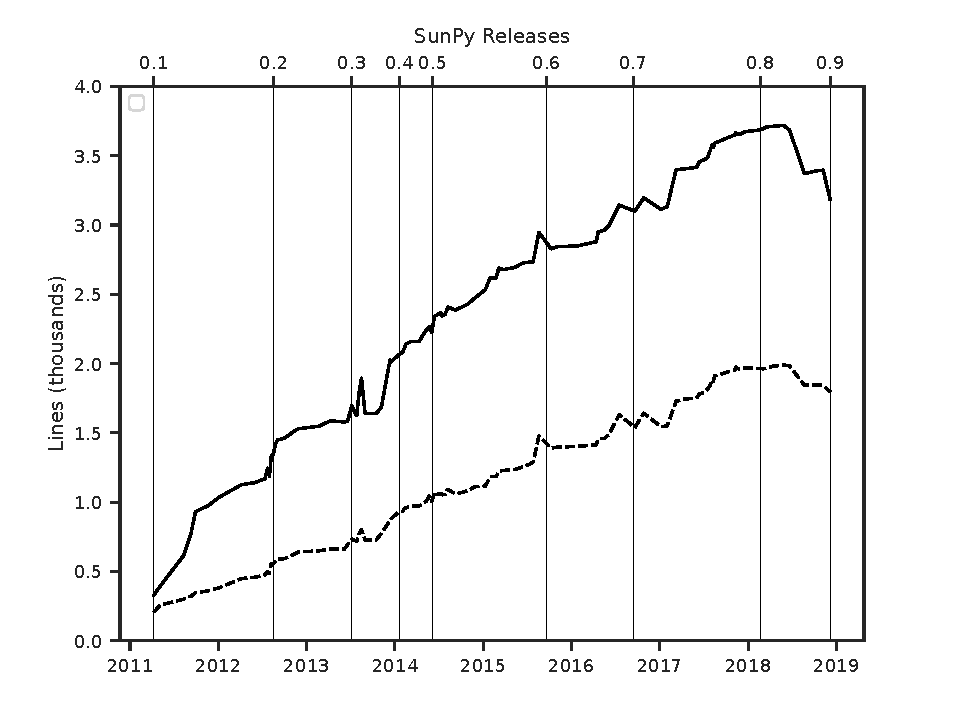
\includegraphics[width=0.5\textwidth]{figures/sunpy_history.pdf} &
  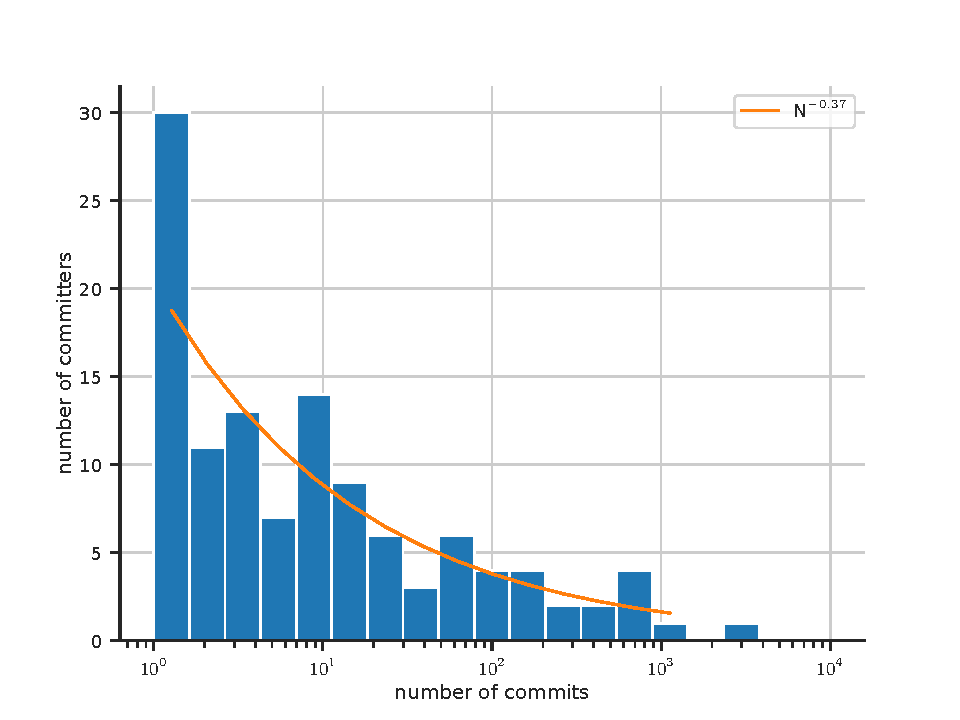
\includegraphics[width=0.5\textwidth]{figures/busfactor_plot.pdf} \\
(a) & (b)  \\
\end{tabular}
\begin{tabular}{c}
  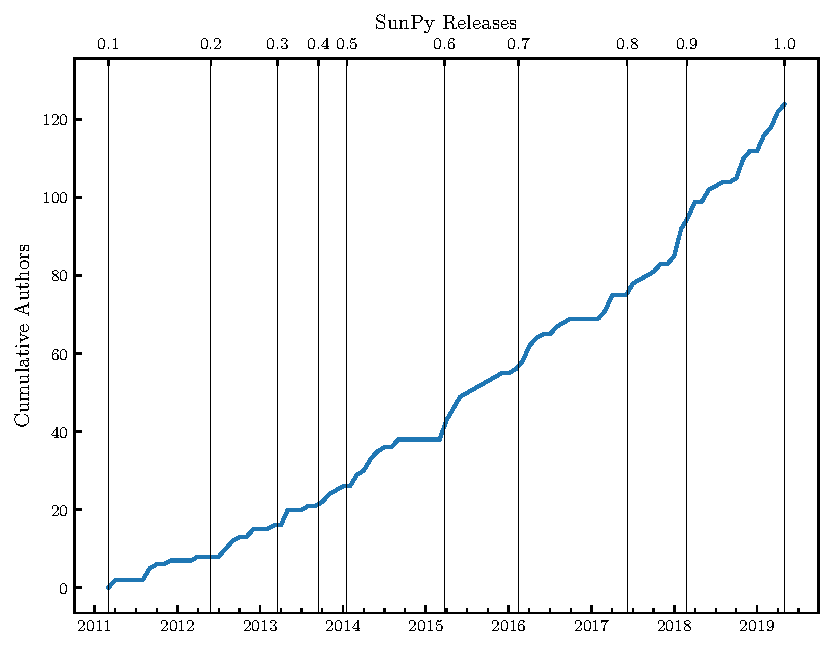
\includegraphics[width=0.5\textwidth]{figures/cumulative_authors.pdf} \\
(c)  \\
\end{tabular}
\caption{
	(a) This figure charts the amount of lines of Python code (dotted black line) and total line count (solid black line) with each major release of \sunpy.
	It details a steady increase of the \sunpypkg codebase with larger additions to our documentation over the last few major versions of \sunpypkg.
	The most striking are the reductions after version 0.9, going into 1.0.
	This was a period that undersaw major phases of code organization, deletion of obsolete features as well as removing Python 2 support.
	(b) This figure showcases the amount of authors to the number of commits they have done.
	It should be noted that the number of commits is not a 100\% useful measure as any one commit could have as many code or line changes as the previous 100 commits.
	However, it does indicate the majority of commits within the package are undertaken by the least amount of people with on average, contributions from an individual is typically less than 10 commits.
	(c) This figure charts the amount of authors (i.e., committers) to the \sunpypkg as a function of time.
	The package has seen a steady rise with time as word of mouth and the community around \sunpy has developed and grown.
	Two periods of time stand out, mid-2015 and early 2018, which saw a large increase in the amount of authors over a shorter period than normal.
}
\label{fig:metafig}
\end{figure}

\section{Data Types - laura}
The \sunpypkg provides core data types that are designed to provide a standardized interface to data structures across data types (images, lightcurves, spectra) as well as data sources. These core data types currently provided by \sunpypkg are \Map and \Timeseries classes which support 2D image data and 1D temporal data, respectively. They offer a consistent interface to the user allowing a simpler work-flow in the analysis and manipulation of observations. These objects provide visualization and basic manipulation routines with a consistent API. For example, metadata is provided by the \code{.meta} property, the data is stored in \code{.data}. They also handle all of the manipulation necessary to read data in from mission-specific files.

This section provides an over of the \Map and \Timeseries objects. 

\subsection{Map - data with two spatial dimensions}
The \Map class provides the functionality to store 2D data associated with a coordinate system and relevant meta data, such as images of the Sun. A \Map object is created using the \Map\ factory which will produce a \GenericMap object or a subclass of \GenericMap which deals with instrument specific data. 






Images from the following instruments are explicitly supported in \sunpypkg. Explicit support means that a \Map\ source file exists for each image source.  The source file provides a compatibility layer between the source science data and the \Map\ object.  This conveniently allows the definition of source-specific parameters, such as color tables. SunPy typically uses the color tables as provided by the instrument team, with appropriate image scaling to account for the dynamic range of the image.
\begin{itemize}
    \item SDO: AIA, HMI line-of-sight magnetograms
    \item SOHO: EIT, MDI
    \item STEREO: EUVI, COR1 and COR2 data from both STEREO-A and STEREO-B
    \item Hinode: XRT
    \item IRIS: Slit jaw imager (SJI) data
    \item KCor: all polarized brightness data.
    \item PROBA2: SWAP
    \item RHESSI: single reconstructed images
    \item TRACE: All single-image FITS files.
    \item Yohkoh: SXT
\end{itemize}
Helioviewer JPEG2000 image files of the above data sources are also supported by the \Map\ class.

\subsection{TimeSeries}
Time-series data is a of the fundamental observational data types. The \Timeseries class is designed to handle time-series data through a robust and consistent interface. The inherent structure of a \Timeseries object consists of times and measurements while the underlying structure used to store the data is a \code{pandas.DataFrame}. It supports time-series data from a wide range of solar instruments. 

The \GenericTimeSeries class is the base class of \Timeseries, which is created through the \Timeseries factory. A number of instruments are supported through subclassing which have instrument-specific methods for reading source files. Custom \Timeseries can also be made from input data in the form of a \code{pandas.DataFrame}, an \code{astropy.table.Table} or a \numpy array. 

\Timeseries currently supports data sources from the following instruments: the Geostationary Operational Environmental Satellite (\textit{GOES}) X-ray Sensor (XRS), \textit{SDO} EUV Variability Experiment (EVE) \citep{woods2010extreme}, \textit{PROBA2} Large Yield Radiometer (LYRA) \citep{dominique2013lyra}, \textit{Fermi} Gamma-ray Burst (GBM) monitor \citep{meegan2009fermi}, the Nobeyama
Radioheliograph (\textit{NoRH}) \citep{nakajima1994nobeyama}, and \textit{RHESSI} \citep{lin2003reuven}. The \Timeseries\ object also supports the National Oceanic and Atmospheric (NOAA) Space Weather Prediction Center (SWPC) solar cycle monthly indices and predicted progression. Similar to \Map, these data sources are supported as there is a \Timeseries\ source file for each listed above. With this strucuture additional instruments and data sources can easily be added. 

\Timeseries holds meta data, stored in the \Timeseriesmetadata object. This functionality is designed to allow the user to create a single \Timeseries by combining multiple \Timeseries together into one, preserving the metadata relevant to each cell, column or row, concatenated into an organized fashion. 

\Timeseries also supports manipulation functionality for working with time-series data including adding new columns of data to a \Timeseries, truncating a \Timeseries over a specified time range, resampling, and creating other data products from an existing \Timeseries, such as into a pandas.Dataframe or an astropy table. The \Timeseries object, similar to \Map, has it's own visualization plotting methods allowing for easy inspection of the data.




\section{Solar Coordinates}
\label{sec:coords}

The \package{sunpy.coordinates} subpackage provides:
\begin{itemize}
    \item A robust framework for working with coordinate systems
    \item Functions to obtain the locations of solar-system bodies
    \item Functions to calculate Sun-specific coordinate information
\end{itemize}
The currently supported Sun-centered coordinate systems are Heliocentric Aries Ecliptic (HAE), Heliocentric Cartesian (HCC), Heliocentric Earth Equatorial (HEEQ), Heliographic Carrington (HGC), Heliographic Stonyhurst (HGS), and Helioprojective Cartesian (HPC) \citep[see][]{2006A&A...449..791T}.
The coordinates framework leverages the \package{astropy.coordinates} subpackage and its \code{SkyCoord} class \citep[see Section 3.3 of][]{astropy2018} by defining the above frames and the transformations between those frames.
A \code{SkyCoord} object specifies both the coordinate frame (e.g., HCC) and a representation of the particular coordinate (e.g., Cartesian coordinates).
Since most frames evolve over time, the \code{SkyCoord} object may also specify the observation time.

The observer-independent coordinate frames -- HAE, HEEQ, HGC, and HGS -- are useful for specifying the locations of features on the Sun or objects (e.g., spacecraft) in interplanetary space.
The commonly used HGS frame is of particular note because it transforms in a straightforward manner to and from the Heliocentric Celestial Reference System (HCRS).
The transformation is the combination of two rotation angles: the time-independent angle between the Sun's rotation axis and the HCRS celestial pole \citep[see][]{2007CeMDA..98..155S} and the time-dependent angle of the central meridian (as seen from Earth) relative to the vernal equinox.
This transformation between HGS and HCRS links the frames defined in \package{sunpy.coordinates} with the the frames defined in \package{astropy.coordinates}, allowing any solar frame to be transformed to and from any astronomical frame (\autoref{fig:transform_graph}).
In fact, HAE is actually implemented in \package{astropy.coordinates} (as \code{HeliocentricMeanEcliptic}), but the shared framework means that it can be used seamlessly in \sunpy.

\begin{figure}
    \centering
    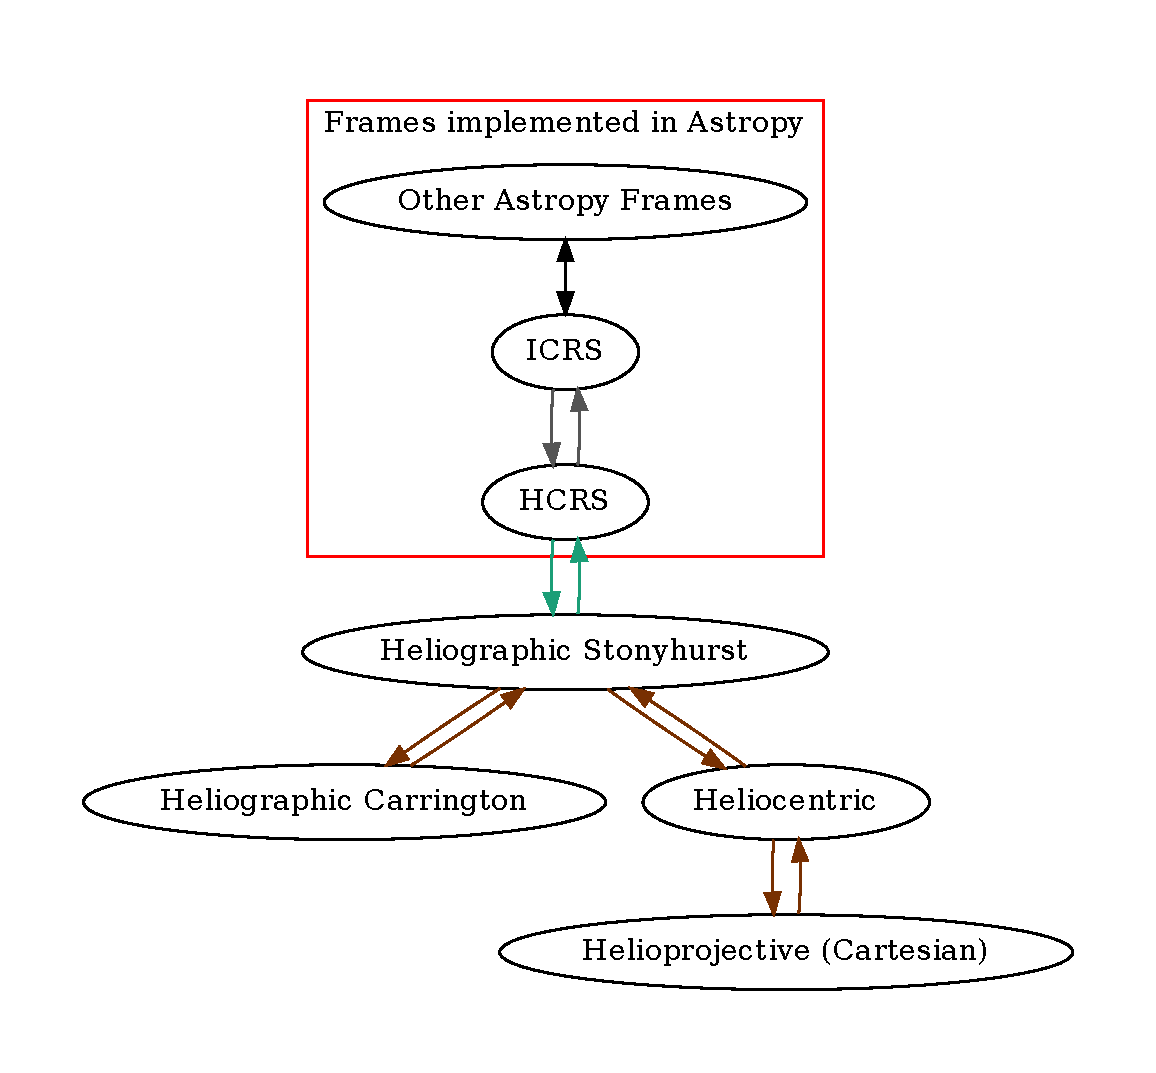
\includegraphics[width=0.75\textwidth]{figures/sunpy_frames.pdf}
    \caption{Graph of the coordinate frames accessible through \package{sunpy.coordinates}, and how they transform between each other.
    The frames within the blue box are actually implemented in \package{astropy.coordinates}, but in the shared framework, any frame can be transformed to any other frame in this graph.}
    \label{fig:transform_graph}
\end{figure}

The observer-dependent coordinate frames -- HCC and HPC -- are useful for observational data, with the potential for subsequent transformation to an observer-independent frame.
The HPC frame in particular is widely used for images from solar missions.
These frames have axes that change orientation depending on the location of the observer, and thus the observer location is necessary to fully define the frame.
This observer location is also stored in the \code{SkyCoord} object.
If the observer is not explicitly specified, the observer is assumed to be at Earth, which may be an adequate approximation for most observations.
Be aware that using the default observer of Earth does not fully define the frame unless the observation time is specified, since the location of Earth needs to be known.

\begin{figure}
    \gridline{\fig{figures/fig_fieldlines_aia.pdf}{0.3\textwidth}{(a)}
              \fig{figures/fig_venus_transit.pdf}{0.3\textwidth}{(b)}
              \fig{figures/fig_coronagraph_starfield.pdf}{0.3\textwidth}{(c)}
              }
    \caption{Several example use cases of the coordinates machinery in \sunpy.
    (a) Field lines traced from a potential field extrapolation overlaid on a 171 \AA{} AIA observation of an active region from 2019 March 10 00:00:04 UTC.
    The field extrapolation was computed with \package{pfsspy} \citep{david_stansby_2019_3237053}.
    (b) The Venus transit as viewed by SDO/AIA in 1600 \AA. The predicted position of Venus is overplotted in the helioprojective coordinate frame of the AIA image.
    (c) A coronagraph image of the solar corona as observed by STEREO-A COR-2. The predicted positions of stars from the Gaia DR2 catalog as well as Mars are overplotted.}
    \label{fig:coordinates_examples}
\end{figure}

The \package{sunpy.coordinates} subpackage enables significant functionality in the \sunpycode{Map} object (see \autoref{sec:map}), and a few examples are shown in \autoref{fig:coordinates_examples}.
The center and rightmost panels of \autoref{fig:coordinates_examples} make use of functions in \package{sunpy.coordinates} to obtain the location of solar-system bodies.
\code{get\_body\_heliographic\_stonyhurst} not only returns the location of one of the planets, but can appropriately correct for light travel time to an observer to return the apparent location (in the past) of that planet.
This planet location is obtained using the active ephemeris in \package{astropy.coordinates}, so if one wants the location of a non-Earth body and accuracy is important, one should use \code{astropy.coordinates.solar\_system\_ephemeris} to specify a JPL ephemeris rather than Astropy's default ephemeris.
\code{get\_horizons\_coord} allows one to query JPL HORIZONS\footnote{\url{https://ssd.jpl.nasa.gov/?horizon}} for the location of a wide range of solar-system bodies.
JPL HORIZONS includes ephemeris information not only for planets and other natural bodies in the solar system, but also for major spacecraft such as SDO and SOHO.
This function requires the \package{astroquery} package \citep{ginsburg_astroquery_2019} to be installed and an Internet connection.

The coordinate framework is also used to calculate Sun-specific coordinate information with high accuracy.
These functions are under \package{sunpy.coordinates.sun} and return values such as Carrington rotation number for the provided time.
Nearly all of the returned values match values in the \textit{Astronomical Almanac} to published precision (e.g., the hundredth of an arcsecond for apparent right ascension).
For times that are provided to these functions, one should take care to specify whether the time scale is UTC or some other time scale (see \autoref{sec:units}).

\subsection{Differential Rotation}
\label{sec:differential_rotation}

%1-2 sentences intro; 1-2 sentences describing what is new; 1 sentence that acknowledges the figure.

% Can delete the first two sentences if the background info feels unnecessary 

When analyzing the dynamics of observed solar emission, it is important to account for variations due to the rotation of the Sun.
In particular, one must account for \textit{differential rotation}, or the latitudinally-varying rotation rate due to the non-rigidity of the solar interior.
The \package{sunpy.physics.differential\_rotation} subpackage provides tools for transforming both \code{SkyCoord} coordinate and \code{Map} objects according to the differential rotation of the Sun.
The amount of rotation can be specified using either a new time, a time interval, or a new observer location.

While earlier versions of \sunpy included tools for dealing with differential rotation, this release includes several improvements.
For example, applying the effect of solar differential rotation now properly accounts for the changing position of the observer.
This can be important because, for example, observers on the Earth must take into account the motion of the Earth in addition to solar differential rotation when calculating how much a location on the Sun appears to move.
\autoref{fig:diff_rot} shows an example using a 1600 \AA{} AIA observation of how differential rotation can be applied to \code{Map} objects.
The image in the middle panel was observed approximately two days after the image in the top panel.
The bottom panel shows the top panel differentially rotated using the observer location and time from the middle panel, showing the good agreement with the actual observation in the middle panel.

\begin{figure}
    \center
    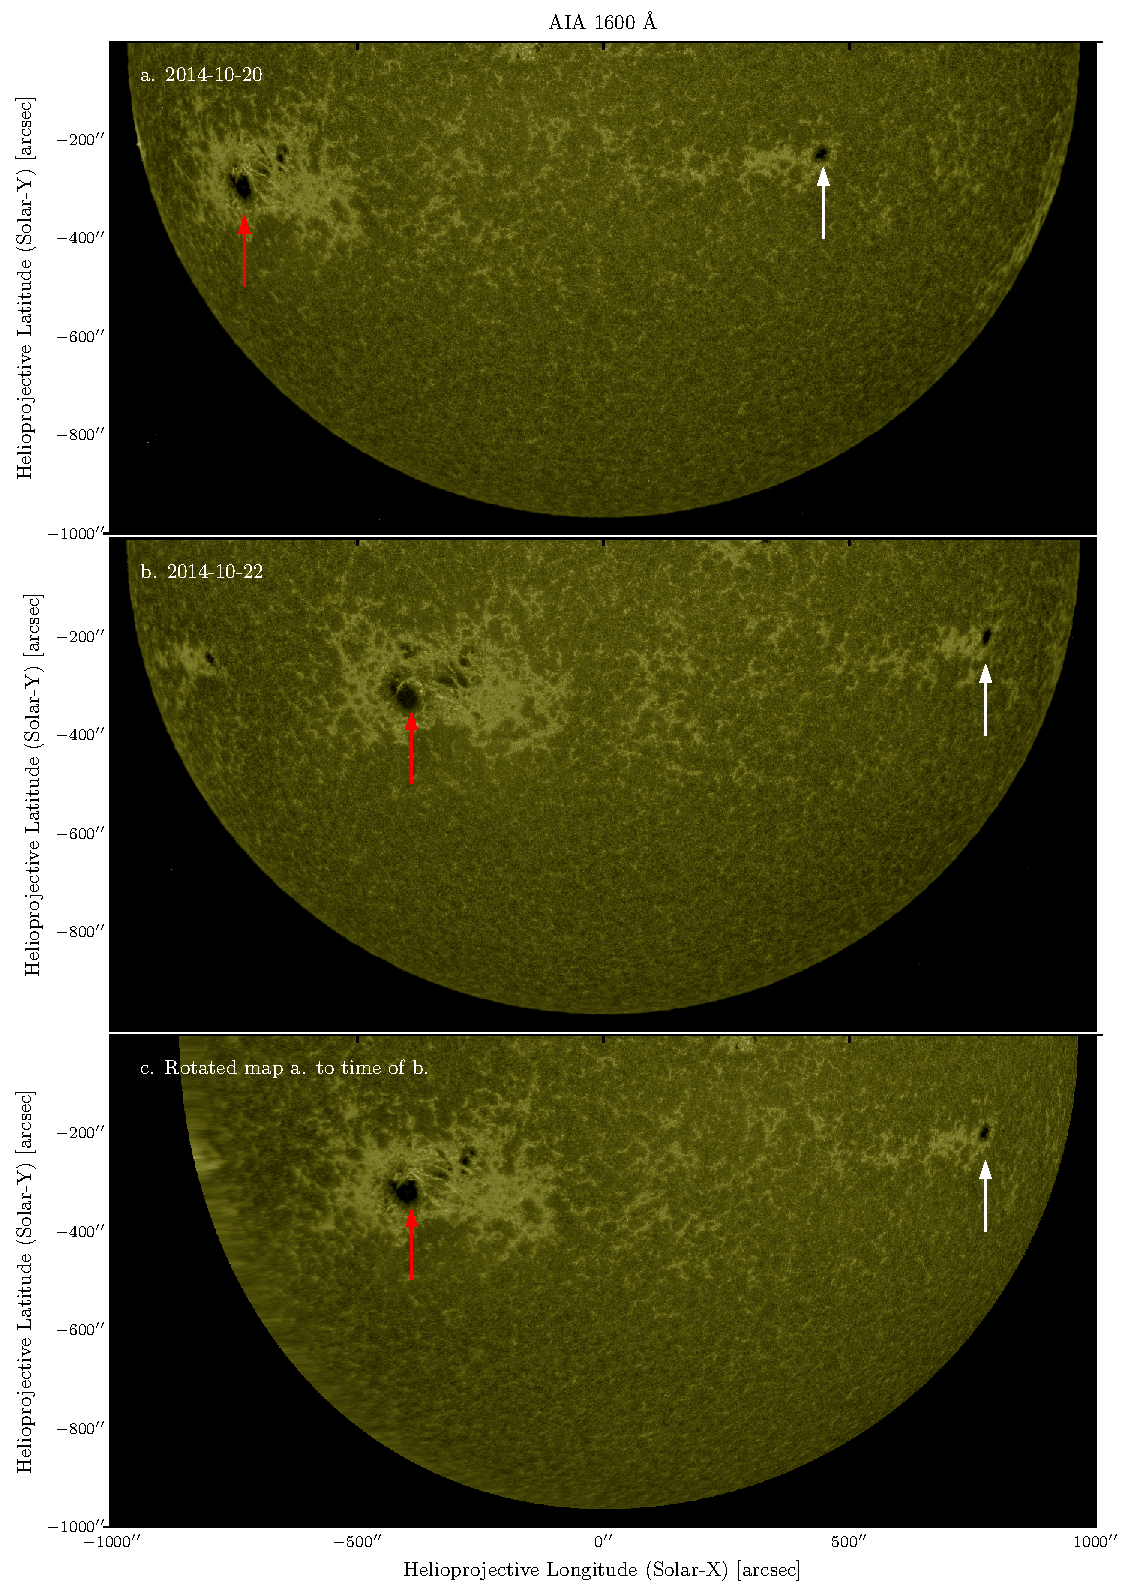
\includegraphics[width = 0.8\textwidth]{figures/fig_diff_rot_1600.pdf}
    \caption{Example of the functionality of \sunpy to apply solar differential rotation to a Map.
    Panels (a) and (b) show the Sun as observed in AIA 1600~\AA\ on two different days, 2014-02-20 and 2014-02-22.
    A large sunspot group is highlighted by the red arrow, and a smaller sunspot by the white arrow.
    Panel (c) shows the map of (a) that has been rotated differentially using \sunpy to the time of map (b).}
    \label{fig:diff_rot}
\end{figure}


\section{Data search and retrieval}
\label{sec:fido}

One of the most important tasks that must occur before any analysis can take place is to search for and retrieve data.
A particular science goal may require data from multiple data providers, each of which may have different methods of search and retrieval.
This heterogeneity increases the effort required by scientists to get the data they need.
In order to address this issue \sunpypkg provides a single and powerful data search and retrieval interface called \Fido. 

\Fido provides a unified interface that simplifies and homogenizes search and retrieval by allowing data to be queried and downloaded from multiple solar sources simultaneously irrespective of the underlying client.
Currently \Fido supports the Virtual Solar Observatory (VSO), the Joint Science Operations Center (JSOC) (see Section \ref{sec:drms}) and a number of individual data providers that make their data available via web-accessible resources such as HTTP websites (RHESSI, SDO-EVE, NOAA GOES soft X-ray flux, PROBA2-LYRA and NOAA sunspot number prediction) and FTP sites (NOAA sunspot number, Nobeyama Radioheliograph).

A \Fido search can include multiple instruments, and can query all available data providers with a single query.
Search queries make use of search attributes (e.g. instrument, time range, wavelength) which can be joined using Boolean operators enabling complex search queries to be constructed easily.
The result of a query can be inspected and edited before retrieval.

The result of the \Fido search query is downloaded via asynchronous download streams significantly improving download speeds.
\Fido also recognizes failed data downloads and allows for re-requesting files which were not retrieved.

In addition to data download, access to event catalogues are also an important aspect of solar physics research. 
The primary solar event catalog is the Heliophysics Event Knowledgebase (HEK) which provides a searchable database of manually and automatically detected solar features and events such as sunspots, solar flares, coronal mass ejections, etc. \sunpypkg provides a HEK search client which is highly flexible, allowing multiple event types and their properties to be queried simultaneously.
For example, it is possible to search for SPoCA (\cite{2014AA...561A..29V}) active regions above a user-specified size within a given time-range.

Finally, \sunpypkg has a Helioviewer\footnote{\url{https://helioviewer.org/}} client which permits the user to query the Helioviewer JPEG2000 image archive, download image data, and easily construct images of solar data from multiple sources available at the Helioviewer archive.
This will eventually  be moved out of \sunpypkg to an affiliated package in order to expands the scope of the client.

\section{Physical Units - Bobra}
\label{sec:units}
\todo{edits by Steven Christe}

%Discuss the units SEP. discuss that we are using astropy units and provide a short description of it's capabilities. mention that sunpy.sun provides quantities with units. mention the NASA units disaster and reference units policy for NASA as reference here is a interesting reference \url{https://sma.nasa.gov/news/safety-messages/safety-message-item/lost-in-translation}

Calculations of physical quantities have traditionally been performed in software 
using bare numbers in the interest of speed as well as simplicity. Physical units
have frequently been recorded in comments or in documentation which can easily lead
to errors and potentially catastrophy. The Mars Climate Orbiter mishap in 1988 was caused by a unit discrepancy. The spacecraft trajectory was reported in English units instead metric which led to the the Mars Climate Orbiter entering the Martian atmosphere well-below its intended altitude causing complete mission failure \citep{mco_mishap_report}. A more modern approach is described by \citep{Damevski2009}
which consists of describing units at the system architecture level. This capability 
is provided by the \package{astropy.units} module and and a SEP mandates its use.

The \package{astropy.units} module defines a \code{astropy.units.Quantity} class which combine a value and a unit. This class is an extension to \code{numpy.array} and provides significant performance compared to other approaches \todo{add a reference here?}. Every input and output of \sunpypkg functions that requires a physical value make use of \code{astropy.units.Quantity}. Enforcement on input is provided by a decorator (\code{quantity\_input()}). This approach eliminates any confusion about the units of a physical quantity in input or output. Also conversions between such as Gauss and Tesla units are made straightforward with the \code{.to()} method.

The \package{sunpy.sun} module contains constants, parameters and models of the Sun provided as \code{astropy.units.Constants} which are \code{astropy.units.Quantity} with additional reference metadata. These include variable quantities, such as the Carrington rotation number, as well as constants, such as the solar mass. 

\todo{do we want to discuss astropy time in this section as well?}


\section{Affiliated Packages - Steven}
\label{sec:affil_package}
In order to foster an interoperable software environment which minimizes the cognitive burden on users, the \sunpy project supports the concept of affiliated packages.
A \sunpy affiliated package is a \python package that builds upon the functionality of the \sunppkg package or provides general functionality useful to solar data analysis. Affiliated packages can also be used to develop and mature core functionality outside of the constraints of \sunppkg.

In order to promote high-quality code and foster consistency and interoperability the following requirements must be satisfied by any potential affiliated packages.
\begin{itemize}
    \item In order to reduce code duplication and complexity, the package must make use of all appropriate features in \sunppkg.
    \item Documentation must be provided that explains the function and use of the package, and it should be of comparable quality to \sunppkg.
    \item A test suite must be provided to verify the correct operation of the package.
    \item The developers should engage with the community to encourage knowledge and code sharing.
\end{itemize}

Developers can formally apply to become an affiliated package to the \sunpy lead developer whose responsibilities include to define the application and review process. Final approval is required of the board for acceptance. Packages are re-reviewed on a yearly basis to ensure that they continue to meet the standards. All affiliated packages are listed on \url{sunpy.org}, provided support by the \sunpy developer community, and further advertised at conferences and workshops. In addition, the project further defines sponsored affiliated package which is an affiliated package whose maintenance and development is the responsibility of the \sunpy project.  

The following section provides short descriptions of the existing affiliated packages.
\label{sec:affil_packages}

\subsection{drms - Kolja Glogowski - MONICA}
\label{sec:drms}

The \package{drms} affiliated package provides functionality which allows for direct access to data hosted by the Joint Science Operations Center (JSOC). This is the primary data center for the Solar Dynamics Observatory’s (SDO)\todo{check if these instruments have already been reference before this section, and make sure that reference are provided} Helioseismic and Magnetic Imager (HMI) and Atmospheric Imaging Assembly (AIA) instruments as well as data from the Solar and Heliospheric Observatory's (SoHO) Michelson Doppler Imager (MDI) instrument. DRMS stands for Data Record Management System, a pSQL database that contains metadata, as well as pointers to image data, for every image taken by AIA, HMI, and MDI. The \package{drms} package provides access to the unique search capabilities of the JSOC which include: metadata search queries, export tailored FITS files and serve these files in a variety of methods, as well as export data as movies and images in various formats.

\todo{schriste - clean up, add more detail on that last sentence, also say what is the JSOC API interface}.

\subsection{ndcube - Dan Ryan}
\package{ndcube} is a free, open-source, community-developed Python package for manipulating N-dimensional coordinate-aware astronomical data.
The package provides a unified API for slicing, visualization, coordinate conversion and inspection of the data, metadata and coordinate transformations.
\texttt{ndcube}'s data classes are not specific to any number or physical type of axis.
It can therefore be used for any data type (e.g. images, spectra, timeseries, etc.) so long as it can represented by an array and a set of World Coordinate System (WCS) transformations.
This makes \texttt{ndcube}'s data classes ideal for subclassing when creating data-type-specific classes while keeping the non-data-type-specific functionalities (e.g. slicing) common between classes.

The \texttt{ndcube} package is composed of two basic data classes, \texttt{NDCube} and \texttt{NDCubeSequence}.
(Note the \texttt{ndcube} package is distinguished from the \texttt{NDCube} data class via capitalization.)
\texttt{NDCube} is for managing a single array and set of WCS transformations, while \texttt{NDCubeSequence} is for handling multiple arrays, each described by their own set of WCS transformations.
They share similar APIs to enable the user to think about their data in an intuitive way, rather than focusing on the format in which that data happens to be stored.

\texttt{NDCube} is subclassed from \texttt{astropy}'s \texttt{NDDdata} class and so provides attributes for a single data array (\texttt{NDCube.data}) and corresponding uncertainty (\texttt{NDCube.uncertainty}) and mask arrays (\texttt{NDCube.mask}).
It also provides attributes for the data unit (\texttt{NDCube.unit}) and metadata (\texttt{NDCube.meta}).
Transformations between the pixel/array indices and real world coordinates can be stored in two ways.
The first is as an \texttt{astropy.wcs.WCS} instance in the \texttt{NDCube.wcs} attribute.
Currently a \texttt{WCS} instance is required.
The WCS framework is standard throughout astronomy and many powerful tools for plotting and performing transformations exist in the \texttt{astropy} which are leveraged by \texttt{ndcube}.
New coordinate transformation tools like \texttt{astropy}'s \texttt{gWCS} (Generalized World Coordinate System) will be incorporated into \texttt{ndcube} in the future.
A second optional method of storing coordinate information is as a dictionary of extra coordinates in the \texttt{NDCube.extra\_coords} attribute.
Each entry stores the coordinate's name, the axis or axes to which it corresponds, and a \texttt{numpy.array} or an \texttt{astropy.unit.Quantity} giving the coordinate value at each location along the relevant axis/axes.
The final attribute is \texttt{NDCube.missing\_axis} which will be discussed below.

One of \texttt{NDCube}'s most useful capabilities is its simple, yet powerful slicing.
Slicing can be performed in array-index-space or using real world coordinates.
\texttt{NDCube} uses Python's native slicing API to crop in array-index-space as can be done for other objects like list, tuples, numpy arrays, astropy Quantities, etc.
However, in the case of \texttt{NDCube}, the slicing in not only applied to data array, but also the uncertainty, mask, WCS transformations and extra coordinates.
This allows users to move closer to the speed of thought during their analysis by freeing them from the tedious, well-understood, but easy-to-mishandle process of slicing all aspects of their data.

It is also possible to crop an \texttt{NDCube} instance using real world coordinates thanks to its \texttt{NDCube.crop\_by\_coords} method.
A user defines the lower and upper bounds of a region of interest along each axis using the real world coordinates of the \texttt{WCS} instance.
The method then determines the smallest rectangular region in array-index-space which encompasses that region of interest.
In addition to \texttt{NDCube.crop\_by\_coords}, there is an analogous \texttt{NDCube.crop\_by\_extra\_coord} method which allows a user to crop an \texttt{NDCube} instance using a single extra coordinate.
As with the array-index-space slicing described above, both the above methods apply the cropping not only to the data, but also the uncertainty, mask, \texttt{WCS} instance and extra coordinates.

When slicing data it is common to reduce the dimensionality of the data when only interested in one point along one of the axes.
This can cause issues if the coordinate transformation of another axis is dependent on information from the reduced axis, e.g.\ latitude and longitude.
For this reason, axes from the WCS instance are never removed, only reduced to a length of 1.
However, the dimensionality of the data, uncertainty and mask are reduced in the normal way.  
This can lead to scenarios where there are more axes in the \texttt{WCS} instance than the data arrays.
To handle this issue, the \texttt{NDCube.missing\_axis} attribute is used.
This is a list boolean values which indicate which axes of the \texttt{WCS} instance do not have a corresponding axis in the data array.  
By referencing \texttt{NDCube.missing\_axis}, the correct WCS transformations can always be made.
In the case of extra coordinates corresponding to a reduced axis, the coordinate value at the location where the axis was sliced is retained, but the extra coordinate's axis is presented as \texttt{None}.

While \texttt{NDCube.extra\_coords} explicitly supplies the value of a coordinate at each location along its associated axis or axes, such values for the coordinates of the \texttt{WCS} instance are stored functionally.
Although this can be very useful, e.g.\ by reducing the size of the object and enabling the use of powerful plotting tools like \texttt{WCSAxes}, there are times when a user wants to extract the coordinate values.
\texttt{NDCube} provides a few methods to conveniently perform these transformations.
\texttt{NDCube.pixel\_to\_world} allows a user to get the real world coordinates of a pixel or multiple pixels by entering their indices along all axes.  \texttt{NDCube.world\_to\_pixel} does the same in reverse.  As with the equivalent native \texttt{astropy.wcs.WCS} method, \texttt{world\_to\_pixel} returns the non-integer index values that precisely correspond to the input real world coordinates.  These methods are very useful in performing the transformations for a few array indices, but can be cumbersome when a user wants to perform the transformations for many or all pixels.  To make this easier, \texttt{NDCube} has a \texttt{axis\_world\_coords} method which returns the real world coordinates at each index along all axes.
The only input required is the name or number of the axis or axes along which the transformations should be performed.  The default is to do this for all axes.

\texttt{NDCube} has a number a helpful inspection properties help the user quickly understand the data within.  The \texttt{NDCube.dimensions} which returns an \texttt{astropy.units.Quantity} instance with the length of each data axis.
The \texttt{NDCube.world\_physical\_axis\_types} gives the physical type of each axis derived on the \texttt{CTYPE} parameters on the \texttt{WCS} instance.  By default the names are complaint with the IVOA UCD1+ controlled vocabulary\footnote{\url{http://www.ivoa.net/documents/REC/UCD/UCDlist-20070402.html}} but can be overridden when subclassing.

Another very helpful capability of \texttt{NDCube} is its built-in visualization suite.  It provides a simple, generic API via the \texttt{NDCube.plot} method which visualizes the data differently depending on user inputs and the number of dimensions.  Either a static line plot or image can be produced for 1- and 2-D data cubes, while animated line plots and images can be produced for data cube of $>$1 dimension.  Users can pick which axis or axes should make up the plot/image axes while other dimensions are animated through using interactive sliders.  This visualization suite is based on sunpy animator classes and is the only part of \texttt{NDCube} that is dependent on sunpy itself.  However, the suite is provided as a mixin class so users who don't want to depend of sunpy or who want to build more specific or powerful visualization suites can do so easily by combining their own mixin with \texttt{NDCube}'s other powerful capabilities.

Many of \texttt{NDCube}'s capabilities, such as its slicing and coordinate transformations, depends on the existence a single data array described by a single set of WCS transformations.
However a single set of WCS transformations may not always adequately describe our data set.
Handling these cases is the role of \texttt{NDCubeSequence}, \texttt{ndcube}'s second main data class.
Fundamentally \texttt{NDCubeSequence} is a list of \texttt{NDCube} instances with the same slicing and visualization APIs as \texttt{NDCube} which enable users to still think of and interact with their data as if were a single cube.
By default, \texttt{NDCubeSequence} effectively adds an extra dimension to the data which is considered perpendicular to the axes of the constituent \texttt{NDCube}s.
For example, say we have a set of images, each described its own set of WCS transformations.
Fine pointing adjustments have been applied to each frame manually which introduce discontinuities between the WCS transformations through time.
Therefore, the data cannot by represented by a single combined set of WCS transformations and hence can't be stored in an \texttt{NDCube}.
However, it can be represented as an \texttt{NDCubeSequence} of 2-D \texttt{NDCube}s where the time axis is now represented by the sequence axis.
The data set will be represented as 3-D and users can still, slice, visualize, and perform coordinate transformations in almost the same way as if the data were still stored in a single data cube.

\texttt{NDCubeSequence} can also handle more complicated versions of this scenario.
Say our set of images do not require fine-scale pointing adjustments, but rather are interrupted by a single pointing manoeuvre.  This means that the data set can be described by two sequential 3-D image cubes, the first with a set of WCS transformations before the pointing manoeuvre and second with one from after.
We would still prefer to think of our data as a single 3-D cube but unlike the above example, the sequence axis is not a truly independent dimension, but rather parallel to the time axes of the constituent \texttt{NDCube}s.
In other words, moving from cube to cube along the sequence dimension is the same moving along the time axis, just in bigger steps, than if we were to move along the time axis within a sub-cube.
\texttt{NDCubeSequence} makes this easy by enabling the user to set the \texttt{common\_axis} attribute to one of the data axes of the constituent \texttt{NDCube}s.
With the \texttt{common\_axis} set, users can choose to slice, visualize and inspect the \texttt{NDCubeSequence} as either a 4-D or 3-D data set thanks to properties and methods such as \texttt{NDCubeSequence.index\_as\_cube} and \texttt{NDCubeSequence.plot\_as\_cube}.


\subsection{radiospectra - David}


\subsection{IRISPy - Dan Ryan}
\package{IRISPy} is a package that provides tools to read, manipulate and visualize data from the Interface Region Imaging Spectrograph (IRIS; \citealt{DePontieu2014}). It provides a set of classes for handling both the slit-jaw imager (SJI) and spectrograph (SG) observations. These link the observations with various forms of supporting data including: measurement uncertainties; units; a data mask to mark pixels with unreliable or unphysical data values; WCS (World Coordinate System) transformations that describe the position, wavelengths and times represented by the pixels; and general metadata. These classes also provide methods for applying a number of calibration routines including exposure time correction and conversion between data number, photons, and energy units. 

%Moreover, because the data unit is linked to the object, it is always obvious what unit the data is in. This saves scientists the hassle of performing important, but laborious and repetitive data conversions and avoid confusion by always tracking the unit of the data through those conversions. This leads to more efficient and accurate science.
\section{Community}
\label{sec:community}

The \sunpy community follows an open development process, wherein everyone is welcome to contribute code, raise issues, and provide feedback.
As detailed in \sunpy Code of Conduct, the community encourages everyone, including newcomers, to join this process, and strives to create an create an open, considerate, and respectful environment for all.
As part of the open development process, the \sunpy community maintains many active daily communication channels.
Users can connect with the community through mailing lists, on an open-source protocol for real-time chat called matrix.org, or by attending weekly telecons.
The \sunpy community also fosters code development for newcomers and experienced programmers alike through tutorials, summer programs, and mentorship.

As of the publication of this paper, the \sunpy community consists 113 contributors, and an average of approximately 200 commits to the code base on a monthly basis.
The commit history for the entire project is openly available, as are statistics for the number and frequency of commits per developer.
Developers and contributors to the \sunpy project receive credit for their work by authorship on papers, posters, and release notes.

\section{Infrastructure}
\label{sec:infrastructure}

\subsection{Release Cycle, Versioning, Long-term Support}
As of the release of 1.0, a formal release schedule for \sunpypkg has been adopted.
Two releases are planned per year with 6 months between each.
In order to align with the release cycle of \astropypkg, a major upstream package, the plan is to release each May and November.
The first release of the year will be a Long Term Support (LTS) release which will be supported for 12 months or until the next LTS release.
The second release will be a non-LTS and will be supported for 6 months or until the next release.
A formal versioning convention has also been adopted going forward.

\sunpypkg will follow the following versioning system: ``X.Y.z", where the three components have the following meaning;
``X" is the LTS version number, which will be incremented with every LTS, 
``Y" is the release counter, this will be 0 for LTS releases and increment for each intermediate non-LTS release,
``z" is the bug fix number, and is to be incremented for any bug-fix releases.

The primary goal of the adoption of this formal release structure is to provide clarity for support of releases as well as improving predictability of codebase changes for users of \sunpypkg.

\subsection{Continuous Integration}
The \sunpyproj follows common practices and makes extensive use of continuous integration which provide automated testing and code change inspection.
All proposed code contributions trigger test suites to be run on a number of free services (e.g. 
\href{https://azure.microsoft.com/en-gb/services/devops/pipelines/}{Microsoft's Azure pipelines},
\href{https://circleci.com}{circleci},
\href{https://codecov.io/}{Codecov}) which integrate into the \github website. 
These services provide the first review of any contribution by running the test suite on each operating system (Windows, Mac, Linux), testing the documentation build, running figure tests, and providing code coverage metrics.
Additionally \href{https://travis-ci.org}{Travis CI} is used to run the entire test suite on a daily cadence.
\sunpypkg's test suite can be broken down into three broad categories: offline, online and figure tests.
Offline test suite checks the majority of the codebase.
Online tests specifically tests code that make use of online data providers (e.g. VSO or JSOC).
These tests depend on the availability of these online services.
Finally, figure tests generate plots and issue failures if they have changed.
This enables high level functionality testing.
These tests coupled with these services are an important tool for maintaining the integrity of the package and makes it easier for new contributors to understand the impact of their changes.

\subsection{Documentation and Gallery}
The \sunpyproj strives to provide up to date, approachable and high quality documentation.
All documentation for \sunpypkg as well as all affiliated packages is written using the commonly-used \code{Sphinx} documentation build system.
This system supports using plain text files with a markup language called \code{reStructuredText} (RST).
The build process converts these files including documentation strings in Python files into HTML, PDF, or LATEX documents.
We make use of the \code{sphinx-gallery} extension to build a gallery of analysis examples as well as the extension \code{sphinx-automodapi} which generates documentation pages that list all of the available classes, functions, and attributes.
Our \href{http://docs.sunpy.org/en/stable/}{online documentation} is automatically built and hosted on \href{https://readthedocs.org/}{Read the Docs} for all releases.
\section{Conclusion}
\label{sec:conclusion}
Development of the \sunpypkg core package has been ongoing for 8 years with the adoption of a formal project structure 5 years ago at the time of writing this paper.
The core package has grown to provide significant functionality for a growing number of users.
Significant additional features are currently missing and either under active development on are planned for future development.
These include support for spectra (one dimensional or multidimensional) and spectral fitting, support for multi-dimensional datasets (e.g. slit spectrographs), and providing a standardized approach to metadata.

The project formalization process which defined a board structure has succeeded in providing stability as well as better recognition in the community.
Through the board significant decisions were able to be made with some level of community consensus such as adopting an official code of conduct\footnote{\url{http://docs.sunpy.org/en/stable/coc.html}} the purpose of which is to ensure that the \sunpy community is positive, inclusive, successful, and growing.
This is achieved by expecting that community members be open, considerate of respectful in all interactions.

The \sunpyproj is now a member of the \python in Heliophysics Community (PyHC)\footnote{\url{heliopython.org}}, whose members contribute to a collection of over fifty \python packages that span every sub-discipline within heliophysics which includes solar physics. The development of the \sunpy package is consistent with the standards established by the community \citep{pyhcStandards} and many members of
the \sunpyproj are explicit signatories. The goal of this group is to coordinate \python development to improve interoperability and efficiency which aligns with the goals of the  \sunpyproj.

There are a number of obstacles to the continued growth and success of the project. The inability of the project to identify any significant and long-term funding stream has already been discussed in Section~\ref{sec:intro:support}. In addition to that, as shown in Figure~\ref{fig:metafig}, the current team of core developer team is relatively small which suggests a lack of robustness to the loss of key developers.
A significant obstacle to the growth of the core developer team is the difficulty in providing the appropriate tools and guidance to users to convert them into active contributors.
Significant additional skills are required of core developers including knowledge of version control,  refactoring code for public use, writing user documentation, and unit testing which are not currently prevalent in the solar community.
The \sunpyproj is considering a number of ways to address this issue including providing webinars, internship opportunities and improving online documentation.

\section{acknowledgements}

We would like to acknowledge financial contributions by Google as part of the Google Summer of Code program.
This work has made use of data from the European Space Agency (ESA) mission {\it Gaia} (\url{https://www.cosmos.esa.int/gaia}), processed by the {\it Gaia} Data Processing and Analysis Consortium (DPAC, \url{https://www.cosmos.esa.int/web/gaia/dpac/consortium}).
Funding for the DPAC has been provided by national institutions, in particular the institutions participating in the {\it Gaia} Multilateral Agreement.


\acknowledgments

We would like to thank the members of the community that have
contributed to \sunpy, that have opened issues and provided feedback, and
have supported the project in a number of different ways.

TODO: Thank GSoC, ESA/SOCIS for studentships, NumFOCUS (and possibly
PSF) for direct funding. Highligh institutions who let their staff work part
FTE on Sunpy as part of their job.

The following individuals would like to recognize support for their personal
contributions. BMS is supported by the NSF grant AST-1715122 and
acknowledges support from the DIRAC Institute in the Department of Astronomy
at the University of Washington. The DIRAC Institute is supported through
generous gifts from the Charles and Lisa Simonyi Fund for Arts and Sciences,
and the Washington Research Foundation.

\software{Astropy \citep{astropy2018}}

\bibliography{bibliography}

\end{document}
